\documentclass[11pt]{article}
\usepackage{graphicx}
\usepackage{float}
\usepackage{hyperref}
\usepackage{natbib}
\usepackage{listings}
\usepackage{xcolor}
\usepackage[dvipsnames]{xcolor}
\usepackage[svgnames]{xcolor}
\usepackage{amsmath} % For the equation* environment
\usepackage{amssymb}

\hypersetup{
    colorlinks=true,
    linkcolor=red,
    filecolor=cyan,      
    urlcolor=orange,
    pdftitle={Overleaf Example},
    pdfpagemode=FullScreen,
    }

\setlength{\textwidth}{6.5in}
\setlength{\headheight}{0in}
\setlength{\textheight}{8.0in}
\setlength{\hoffset}{0in}
\setlength{\voffset}{0in}
\setlength{\oddsidemargin}{0in}
\setlength{\evensidemargin}{0in}

\lstdefinestyle{txtstyle}{
    basicstyle=\ttfamily\small,
    breaklines=true,
    backgroundcolor=\color{Bisque}
}
\lstset{style = txtstyle}

\definecolor{codegreen}{rgb}{0,0.6,0}
\definecolor{codegray}{rgb}{0.5,0.5,0.5}
\definecolor{codepurple}{rgb}{0.58,0,0.82}
\definecolor{backcolour}{rgb}{0.95,0.95,0.92}

\lstdefinestyle{mystyle}{
    backgroundcolor=\color{backcolour},   
    commentstyle=\color{codegreen},
    keywordstyle=\color{magenta},
    numberstyle=\tiny\color{codegray},
    stringstyle=\color{codepurple},
    basicstyle=\ttfamily\footnotesize,
    breakatwhitespace=false,         
    breaklines=true,                 
    captionpos=b,                    
    keepspaces=true,                                   
    numbersep=5pt,                  
    showspaces=false,                
    showstringspaces=false,
    showtabs=false,                  
    tabsize=2
}

\title{Computational Physics ps-5 Report}
  
\author{Tongzhou Wang, \\ GitHub account: TZW56203, repository: phys-ga2000. \\ \url{https://github.com/TZW56203/phys-ga2000}}

\date{October 6, 2024}

\begin{document}

\maketitle

\section{Problem 1}
The analytical formula for the derivative $f(x) = 1 + \frac{1}{2} \tanh 2x$ is 
\begin{equation}
    f^{\prime}(x) = \frac{1}{\cosh^{2}2x}.
\end{equation}

The numerical derivatives computed using central difference and \texttt{jax} are shown in Figure \ref{fig:central} and \ref{fig:jax} respectively.
\begin{figure}[H]
    \centering
    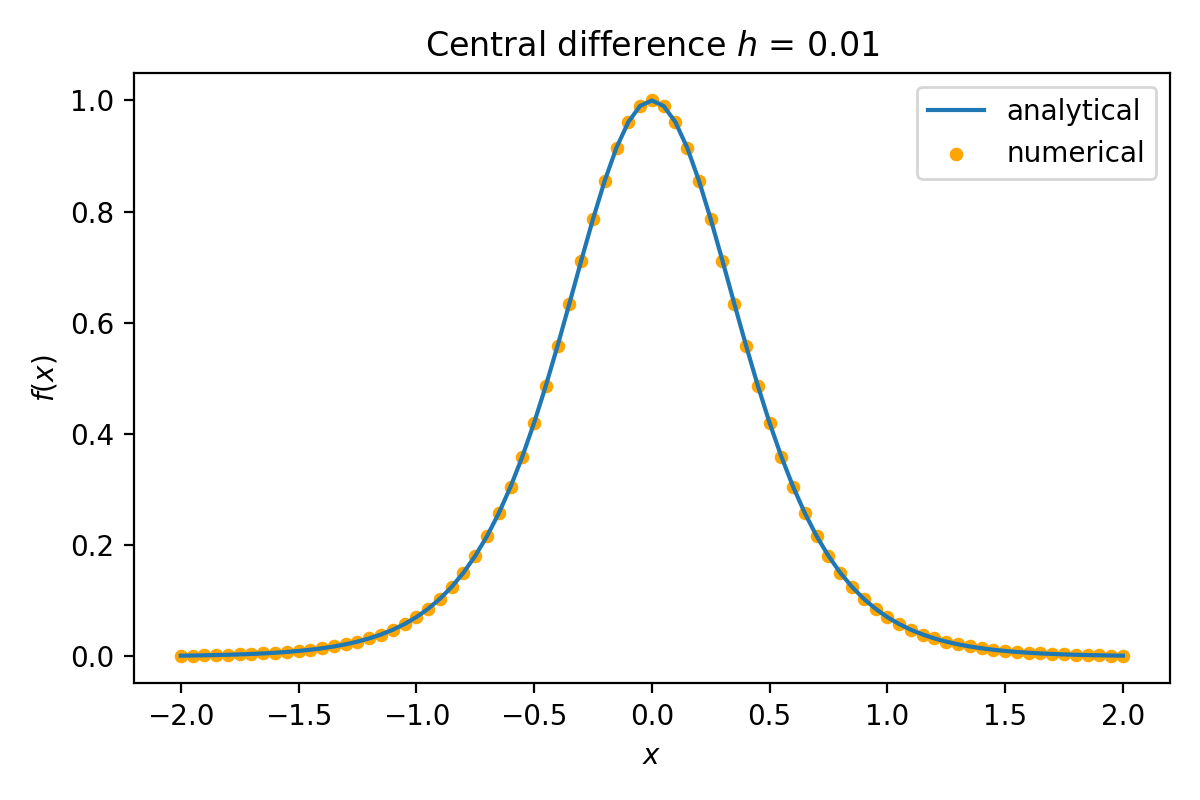
\includegraphics[scale = 0.8]{images/ps-5-1a.png}
    \caption{Derivative computed using central difference.}
    \label{fig:central}
\end{figure}
\begin{figure}[H]
    \centering
    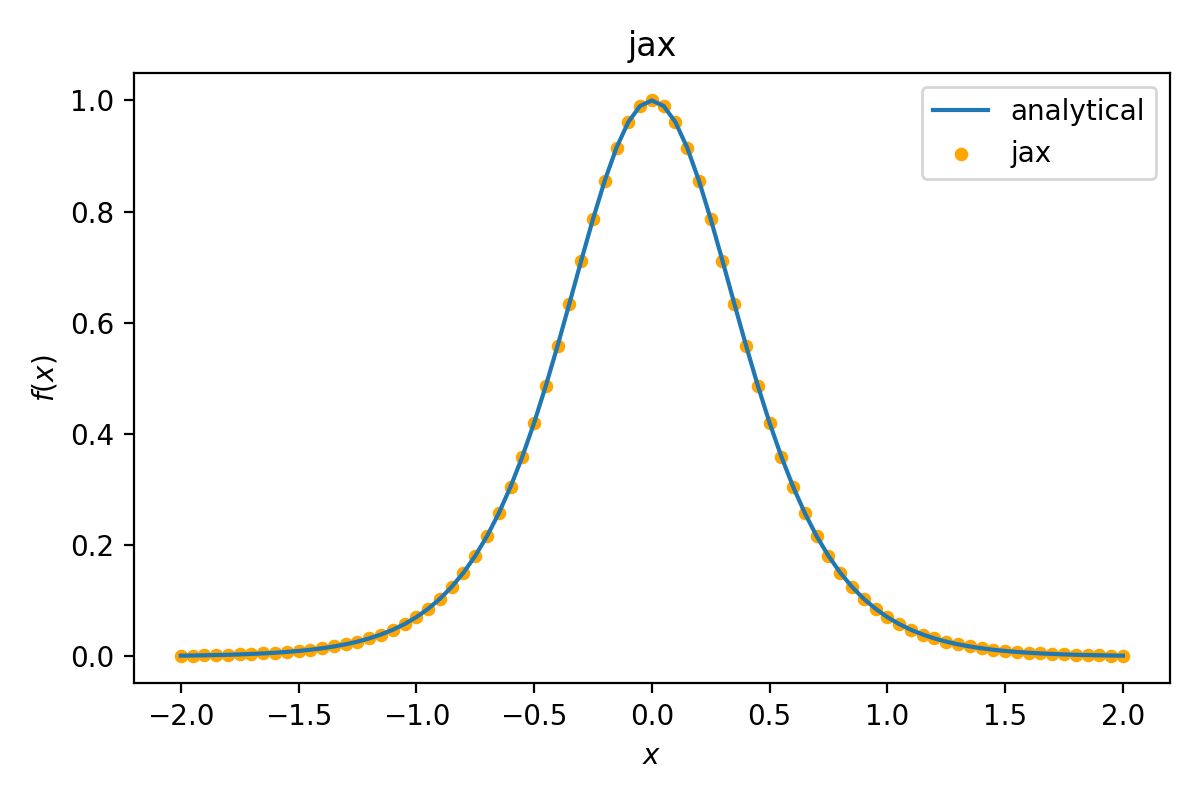
\includegraphics[scale = 0.8]{images/ps-5-1b.png}
    \caption{Derivative computed using \texttt{jax}.}
    \label{fig:jax}
\end{figure}

Listing \ref{lst:derivative} shows that \texttt{jax} seems to be more accurate then central difference in this particular case.
\lstinputlisting[caption={Some values of the derivative.}, label={lst:derivative}]{code/ps-5-1.txt}

\section{Problem 2}
\subsection{Part (a)}
Figure \ref{fig:integrand} plots the integrand of the gamma function.
\begin{figure}[H]
    \centering
    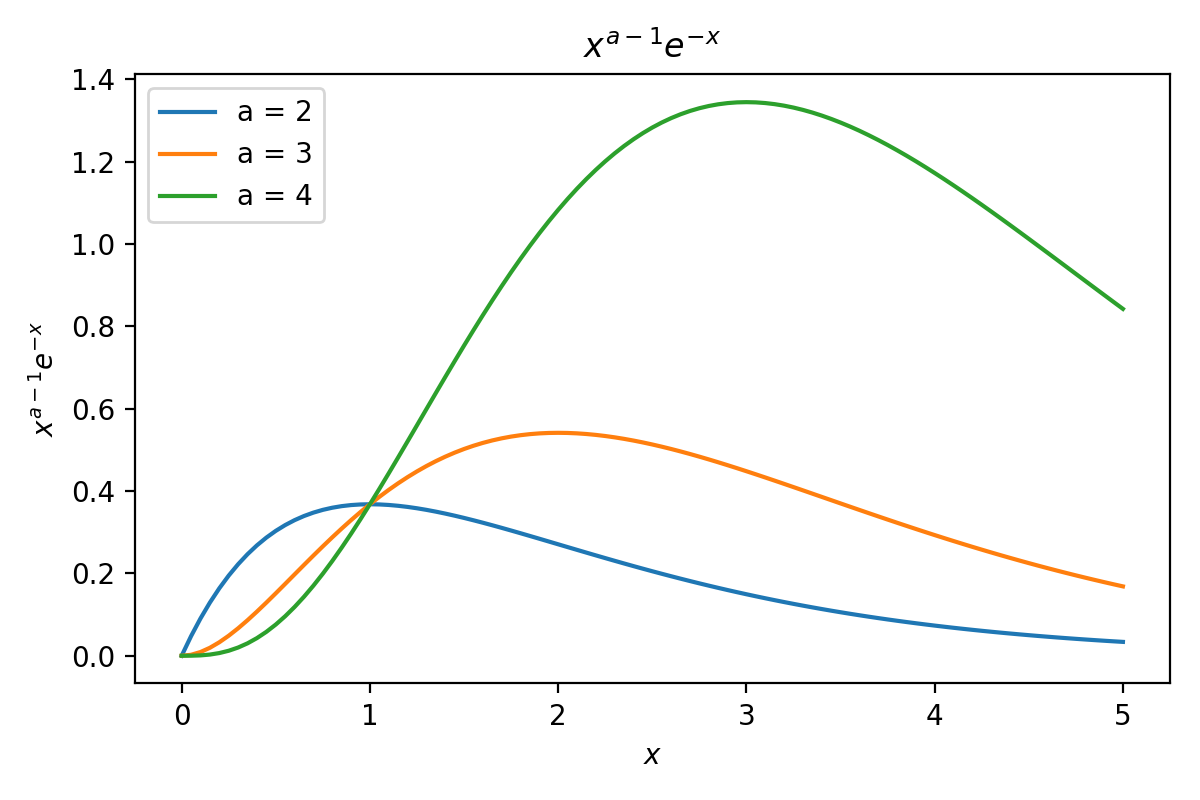
\includegraphics[scale = 0.8]{images/ps-5-2a.png}
    \caption{Integrand of the gamma function.}
    \label{fig:integrand}
\end{figure}

\subsection{Part (b)}
The derivative of $f(x) = x^{a-1}e^{-x}$ is
\begin{equation}
    f^{\prime}(x) = (a-1-x)x^{a-2}e^{-x}.
\end{equation}

Setting $f^{\prime}(x) = 0$, we get $x = 0, (a-1)$.

The second derivative is
\begin{equation}
    f^{\prime\prime}(x) = -x^{a-2}e^{-x} + (a-1-x)(a-2)x^{a-3}e^{-x} - (a-1-x)x^{a-2}e^{-x}.
\end{equation}
Since the integral in the gamma function is from 0 to $\infty$, we assume that $x = a - 1 > 0$. Thus, we have
\begin{equation}
    f^{\prime\prime}(a-1) = -(a-1)^{a-2}e^{a-1} > 0,
\end{equation}
and hence $f(x)$ has a maximum at $x = a-1$.

\subsection{Part (c)}
Obviously, if $x = c$, then $z = \frac{x}{c + x} = \frac{1}{2}$. Hence choosing $c = a-1$ will put the peak of the integrand for the gamma function at $z = \frac{1}{2}$.

\subsection{Part (d)}
We can also express the integrand as
\begin{equation}
\begin{split}
    f(x) & = x^{a-1}e^{-x} \\
    & = e^{(a-1)\ln(x)}e^{-x} \\
    & = e^{(a-1)\ln(x) - x}.
\end{split}
\end{equation}
In the original expression, for large $x$, $x^{a-1}$ may cause overflow and $e^{-x}$ may cause underflow. The advantage of the new expression is that the $\ln(x)$ and $x$ are less likely to cause these issues.

\subsection{Part (e) and (f)}
Listing \ref{lst:gamma} shows the computed values of the gamma function at some points.
\lstinputlisting[caption={Some values of the gamma function.}, label={lst:gamma}]{code/ps-5-2.txt}

\section{Problem 3}
\subsection{Part (a)}
Figure \ref{fig:data} plots the data.
\begin{figure}[H]
    \centering
    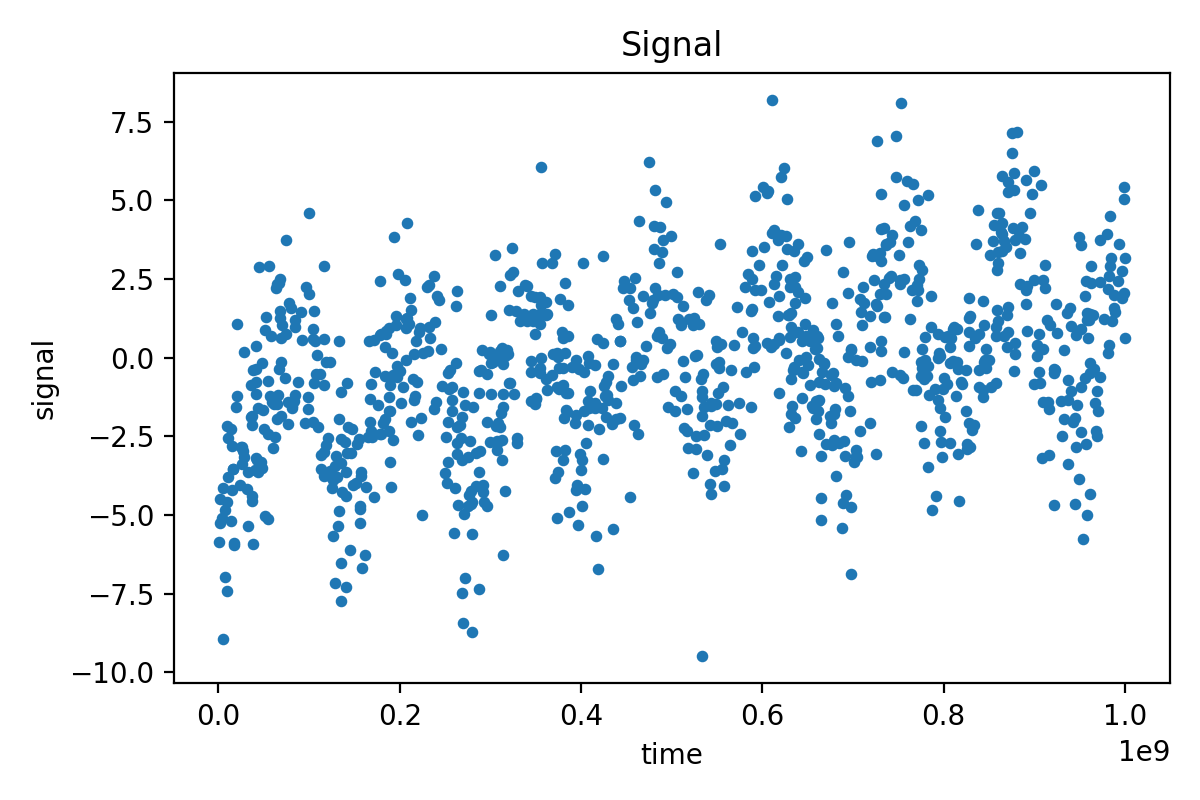
\includegraphics[scale = 0.7]{images/ps-5-3a.png}
    \caption{Plot of the data.}
    \label{fig:data}
\end{figure}

\subsection{Part (b)}
Figure \ref{fig:3order} shows the SVD 3rd-order polynomial fit.
\begin{figure}[H]
    \centering
    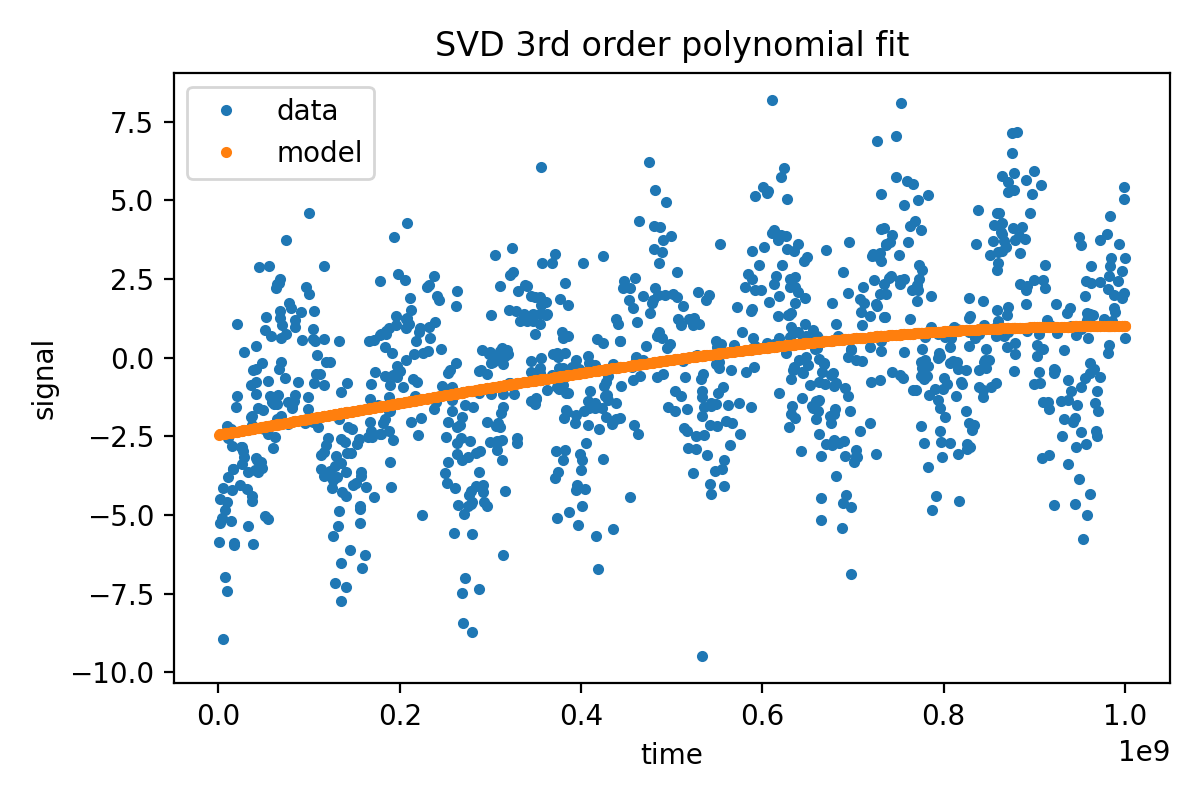
\includegraphics[scale = 0.7]{images/ps-5-3b.png}
    \caption{SVD 3rd-order polynomial fit.}
    \label{fig:3order}
\end{figure}

\subsection{Part (c)}
Listing \ref{lst:residue} shows the condition numbers and residues of the fits performed in this problem. The 3rd-order polynomial fit is not a good explanation of the data because the residue is a bit large. Specifically, its $r / \sqrt{N}$ is greater than the uncertainty of the measurements, which is 2.0.

\lstinputlisting[caption={Condition numbers and residues of the SVD 3rd-order polynomial fit, 23th-order polynomial fit, 21-term Fourier series fit, and 300-term Fourier series fit.}, label={lst:residue}]{code/ps-5-3.txt}

\subsection{Part (d)}
Figure \ref{fig:23order} shows the SVD 23th-order polynomial fit. This is a more reasonable polynomial fit that is a better explanation of the data.

"When the condition number exceeds the dynamic range of your floating point numbers, there is no guarantee that the SVD solution will be stable. Basically, round-off error can then cause the procedure to fail."

As shown in Listing \ref{lst:residue}, the conditional number for the 23th-order polynomial fit is not too large comparing to the dynamic range. And its residue is smaller.
\begin{figure}[H]
    \centering
    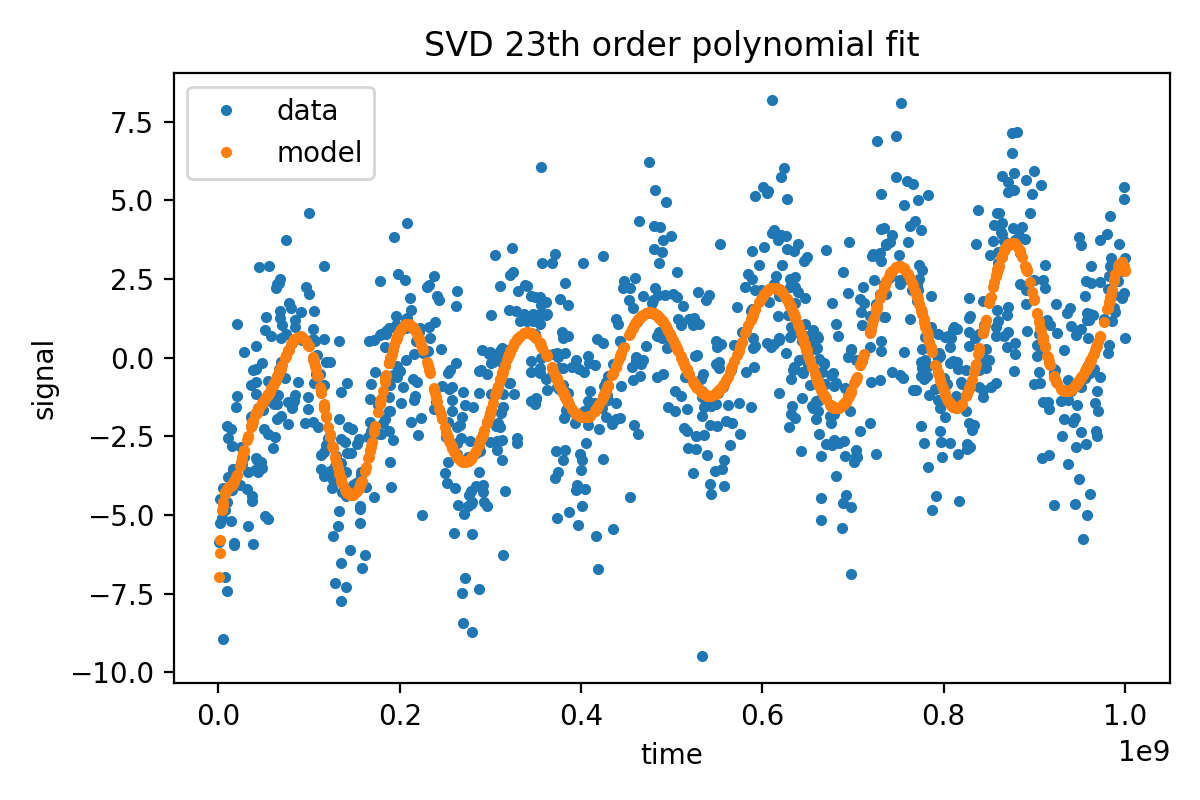
\includegraphics[scale = 0.7]{images/ps-5-3d.png}
    \caption{SVD 23th-order polynomial fit.}
    \label{fig:23order}
\end{figure}

\subsection{Part (e)}
Figure \ref{fig:21term} and \ref{fig:300term} show the SVD 21-term and 300-term Fourier series fits respectively. 

The models do a good job explaining the data. As shown in Listing \ref{lst:residue}, both fits have condition numbers that are small enough to be reasonable. And the 300-term Fourier series fits has smaller residue.

From figure \ref{fig:data}, we can notice a typical periodicity about $T \approx 1.35 \times 10^8$ unit time.
\begin{figure}[H]
    \centering
    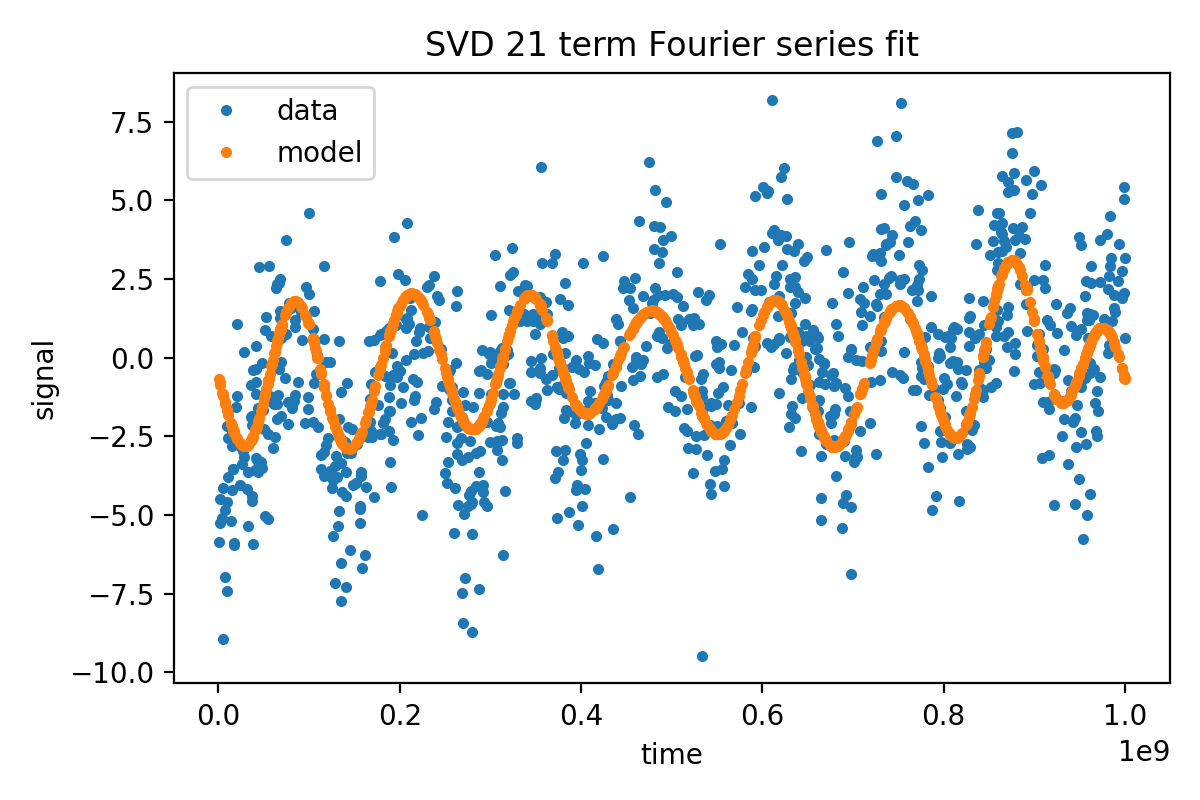
\includegraphics[scale = 0.7]{images/ps-5-3e.png}
    \caption{SVD 21-term Fourier series fit.}
    \label{fig:21term}
\end{figure}
\begin{figure}[H]
    \centering
    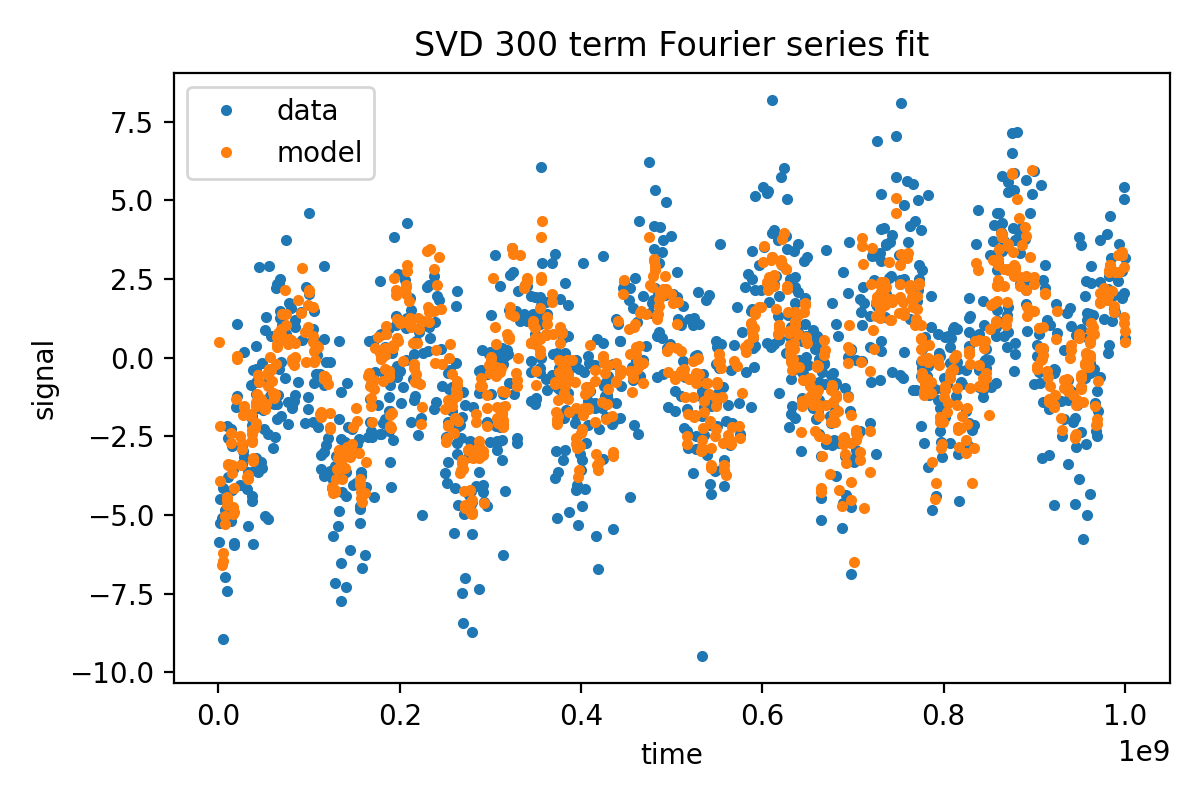
\includegraphics[scale = 0.7]{images/ps-5-3e2.png}
    \caption{SVD 300-term Fourier series fit.}
    \label{fig:300term}
\end{figure}


\end{document}


